\section{Experiment Setup}
In order to valdate the efficacy of my system, I have chosen to compare the output
tertiary structures to literature baselines from \cite{Hoque}. I have chosen
to use the results from this study because they are directly comparable
to my model as the proteins were also optimised on a 3D FCC lattice.
In order to compare candidate lattice structures to real proteins
from the PDB, real proteins from the PDB are first normalized to fit
into a lattice and evironment and then the euclidean distance between the alpha carbon atoms
of the candidate and true structures are calculated, a lower distance indicates
a more accurate prediction.

The following proteins were chosen of varying length in order
to demonstrate the scalability of the architecture I have chosen to implement,
their respective PDB ID and lengths are given in the following table:
\begin{table}[!htb]
    \begin{center}
        \caption{Proteins used for training}
\begin{tabular}{||c | c||}
    \hline
    ID & Length\\
    \hline\hline
    1PJF  & 46  \\ 
    \hline
    2CRT & 60  \\
    \hline
    2FFW & 78 \\
    \hline
    1GH1 & 90  \\
    \hline
\end{tabular}
\end{center}
\end{table}
\section{Results}
The system was unable to generate optimised tertiary strutures.
Despite the average loss for all agents converging, inidicating that
learning was taking place, the actual structures produced faired no
better than random. The system was tested against all 4 mentioned proteins,
no experiment proved to be successful, as a result I was unable to compare
the afore mentioned proteins to their true structures from the PDB.
A training run for each of the proteins is shown below,
the figures track the average reward and loss for each peptide:

\begin{figure}[!htb]
    \centering     
    \subfigure[1GH1]{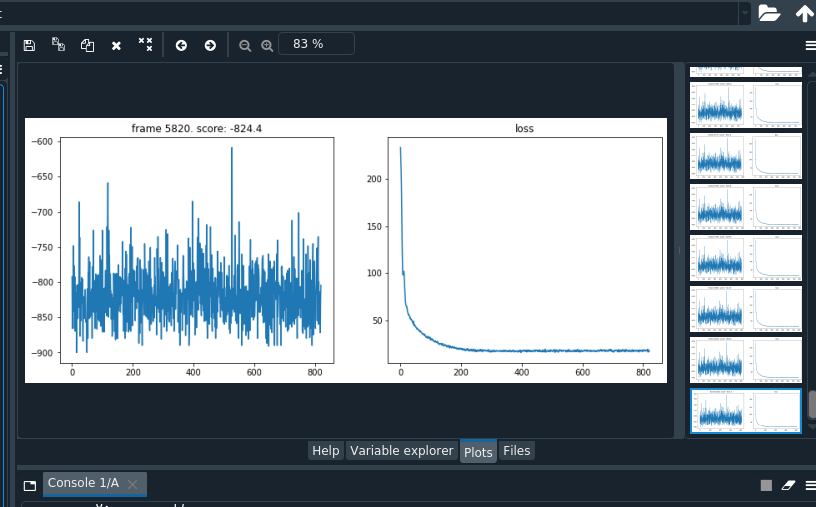
\includegraphics[width=60mm]{Figures/1gh1.png}}
    \subfigure[1PJF]{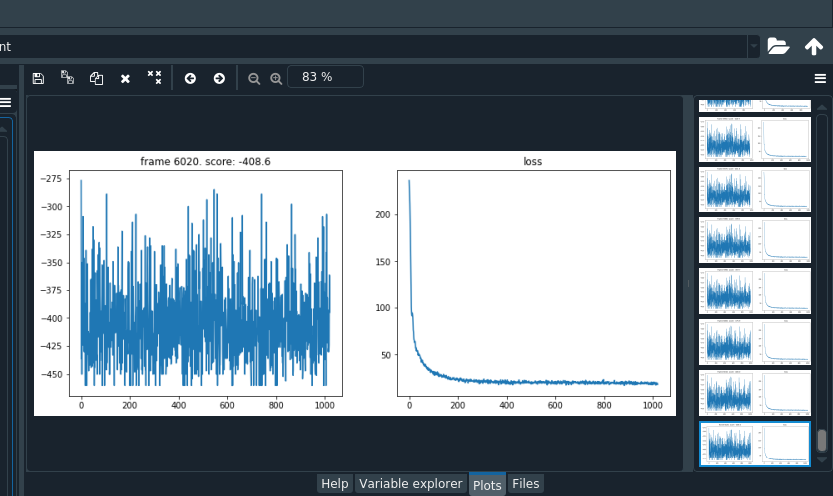
\includegraphics[width=60mm]{Figures/1pjf.png}}
    \subfigure[2CRT]{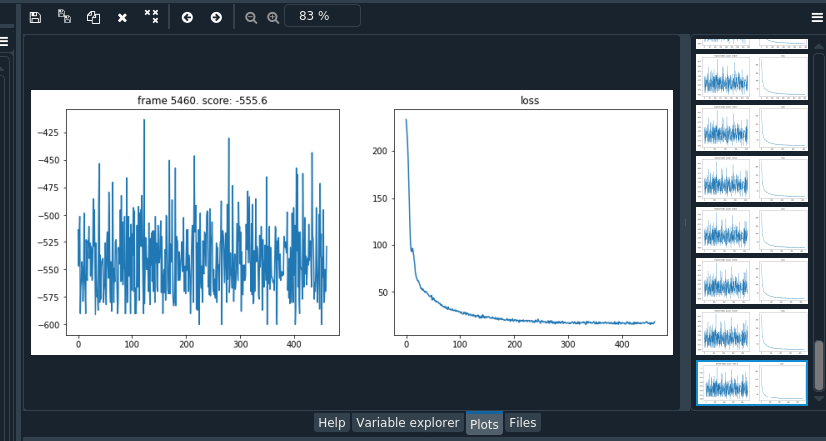
\includegraphics[width=60mm]{Figures/2crt.png}}
    \subfigure[2FFW]{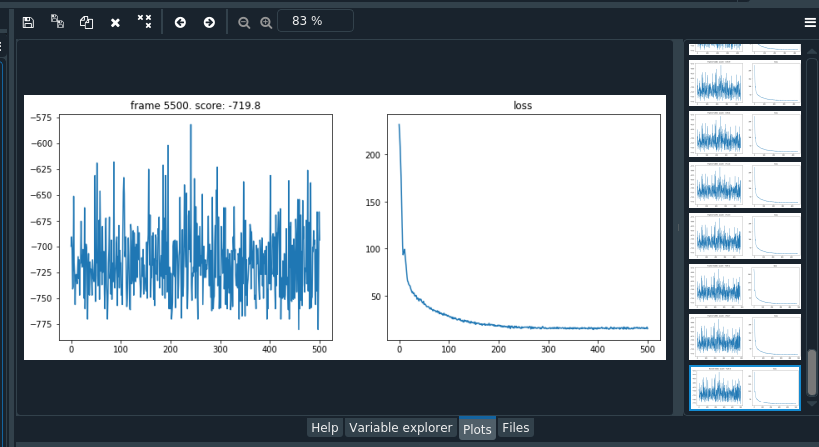
\includegraphics[width=60mm]{Figures/2ffw.png}}
    \caption{Training run for each of the peptides.}
\end{figure}

Longer training runs were recorded using a service called Weights \& Biases
and can be found at \url{https://app.wandb.ai/honne23/mean-field/overview?workspace=user-honne23}.

\subsection{Environment}
The environment was successfully implemented as a 3D FCC Bravais lattice.
The environment successfully reports each residues immediate neighbours
on the lattice while enforcing the integrity of the torsion backbone
by calculating the euclidean distance between the current residue and
its immediate neighbours. The environment can easily be edited
to accomodate different lattice structures by changing the constants
within the Bravais matrix.

I experimented with various penalty structures in order to
promote learning in the environment, none of which were successful.
I tried multiple reward strategies in order to encourage learning:
\begin{enumerate}
    \item Setting a constant reward of -10 for actions
    which broke the self-avoiding-walk (SAW).
    \item Adding -10 to the total reward at local sites on the lattice.
    \item Rewarding all agents only with their immediate local rewards.
    \item Rewarding all agents with the global reward (sum of all local rewards).
    \item Rewarding all agents with the average of all local rewards.
\end{enumerate}
Strategies 3-5 were tried in combination with strategy 1 or 2, none of which
were successful. When none of the reward strategies were shown to work
I tried to set different initialisation conditions. At first,
all proteins were initialised as a straight line in space but
the drawback of this approach was that at the beginning of trainnig,
the only neighbours a residue would have access to are it's immediate
neighbours on the torsion backbone. In addition to this,
because the shaped reward takes into account the
covariance of the coordinates of all residues, when they
were initialised as a straightline in space, the covariance
calculation would evaluate to 0.

In an attempt to remedy this, I instead implemented
\emph{exploring starts} \cite{sutton2018reinforcement}. Exploring
starts is a method of initialisation that starts the agents in
random starting positions in the envrionment rather than the initial
fixed position. I constrcuted the exploring starts as random self
avoid walk on the lattice. Each time the environment was reset,
the residues were initialised to a new random conformation,
this had the added benefit of being able to take advantage of the 
shaped reward although this did not improve training results.


\subsection{Quantile Rainbow Agent}
In order to test my implementation of the rainbow quantile
agent, I first trained it using the OpenAI Gym framework
on Atari games. The agent was shown to be able to learn
the game Pong in a reasonable amount of time. This
agent was later integrated into the mean-field framework
following the procedure elaborated upon in \textbf{System Design \& Analysis}.
Eventhough this model appeared to work in the single agent
setting it was not effective in the multi-agent scenario.
Despite this, the average loss appeared to converge across
all agents, indicating that although learning was taking place,
the agents could not learn any useful strategies.

The core issue appears to stem from the non-stationarity of
the environment from the perspecive of the individual agents.
The transition and rewards of all agents depends on the 
policies of all other agents whch are continuously changing
during the learning process \cite{Papoudakis2019}. While regular deep Q learning
appears to converge in multi agent scenarios, the
quantile rainbow agent was not able to overcome this limitation.


\subsection{Mean Field Multi-Agent Learning}
As the original implementation was in Tensorflow and
mine was in Pytorch, I was unable to test the original 
code from the authors. However, the codebase was
implemented line for line from the original 
implementation with a few notable exceptions.

\begin{itemize}
    \item The original implementation uses a convolutional
    neural network (CNN) to process input from the environment, whereas
    my implementation uses a linear multi-layer perceptron (MLP) instead.

    The drawback of my implentation is that is does not exploit
    spatial coherance the same way a CNN would, this could be one
    of the factors that prohibited successful outcomes during training.

    \item The original implementation also contains an additional
    embedding layer that takes the the types of the agents as input
    and produces a vector embedding that is fed into the rest of 
    the computation. I did not introduce this embedding layer
    in my implementation as its role was unclear and not referred 
    to in the original publication,
\end{itemize}

Other than these exceptions, there were also numerous elements
in the author's implementation that were not referred to in their original
publication. This included an additional embedding layer that
processed the action distribution of layers as well as the 
settings of various parameters such as the range of values used
for the Boltzmann constant $\beta$, steps per weight update and the
learning rate $\tau$. This information was only uncovered after
extensive inspection of the original github repository. 
Even so, after updating my system my agents were still unable
to perform well during training, often resetting the environment after
a 1-4 steps as the torsion backbone would repeatedly be broken,
this prevented the agents from experiencing many possible states,
a problem that unfortunately was not alleviated by utilising
exploring starts.

From further inspection, I beleive the core of the issue 
was the the size of the action space. As mentioned in \textbf{System Design \& Analysis},
each agent has access to $3^3 = 27$ possible actions; consequently
each agent would produce a 27 possible quantile distributions
when considering the next possible action it should take, the result is a $27 \times 51$ matrix
as each quantile distribution was placed on a support of 51 atoms.
In order to weight each quantile distribution appropriately
under the mean field regime each of the predicted quantile
distributions is weighted by the distribution over
neighbouring actions:
\begin{equation}
    Z^*(s,a^j, a^{-j}) = \pi^j_t(a^j \mid s',a^{-j}) \cdot \mathbb{E}_{a^j \backsim(\mathbf{a}^{-j}), Z_\theta \backsim Z}[\hat{Z}(s,a^j, a^{-j})]
\end{equation}

Due to the structure of the lattice, a residue's
immediate neighbours will only be the two it is
connected to along the torsion backbone. 
As a result $\pi^j_t(a^j \mid s',a^{-j})$ would take
on the form of a column vector with values equal
to 0 at all indexes with the exception of the 
indexes of the actions taken by the residues
only two neighbours. The core issue was that
each residue would only have access to the actions 
taken by its immediate neighbours, this highly
constrained the sample size of actions and also
restricted each agent to the actions taken by its neighbours,
greatly inhibiting their learning ability. 
Consider the following
example:
\begin{equation}
    \begin{gathered}
        \pi^j_t(a^j \mid s',a^{-j}) \cdot \mathbb{E}_{a^j \backsim(\mathbf{a}^{-j}), Z_\theta \backsim Z}[\hat{Z}(s,a^j, a^{-j})] = \\
        \begin{bmatrix}
            0.5\\0\\0\\\vdots\\0\\0.5\\0
        \end{bmatrix} \cdot 
        \begin{bmatrix}
            0.5 & 1.1 & 2.2 & \hdots\\
            0.3 & 1.8 & 2.8 & \hdots\\
            0.9 & 1.25 & 2.3 & \hdots\\
            \vdots & \vdots & \vdots & \vdots\\
            0.62 & 1.1 & 2.2 & \hdots\\
            0.48 & 1.8 & 2.33 & \hdots\\
            0.7 & 1.05 & 2.68 & \hdots\\
        \end{bmatrix} = \begin{bmatrix}
            0.25 & 0.55 & 1.1 & \hdots\\
            0 & 0 & 0 & \hdots\\
            0 & 0 & 0 & \hdots\\
            \vdots & \vdots & \vdots & \vdots\\
            0 & 0 & 0 & \hdots\\
            0.24 & 0.9 & 1.165 & \hdots\\
            0 & 0 & 0 & \hdots\\
        \end{bmatrix}
    \end{gathered}
\end{equation}
Most of the distributions evaluate to 0,
which prevents the $\arg \max$ operation from accurately selecting an action.






